\subsection{Smith normal form}

% To obtain the most general invariants, we take $R$ to be $\Z[t, t^{-1}]$, the ring of Laurent polynomials with integer coefficients. However, this ring is not a principal ideal domain 
% the ring $R$ is not a PID but $\Z[\Z]$. It is possible to find invariants over this particular ring, however it is often beneficial to find a PID ring $P$ and send $t\in \Z[\Z]$ to some unit of $P$. 
%
% % Take $P=\Q[\Z]$ and consider a matrix $A\in K\phi$ as a matrix with terms in $P$-module.
The ring $R$ over which we consider modules $M$ is not necessary a principal ideal domain. However, there are plenty of PID rings and one can find at least one PID $P$ with a homomorphism $R\to P$ that allows to consider $M$ as a $P$-module by tensoring it with $P$:
$$M_P=M\otimes_R P.$$
That way, we can consider a new type of equivalence relation on any color checking matrix $D\phi$.
% However, there are plenty of PID rings and one can take any unit of $R$ and send it to any unit of a PID ring $P$ to allow for $M$ and $N$ to be considered as $P$-modules. That way, we can consider a new type of equivalence relation on any color checking matrix $D\phi$.
\begin{definition}[Smith normal form]
Take $A\in K\phi$ and consider it as a $s\times x$ matrix with terms in a $P$. Then there exist a $s\times s$ matrix $S$ and $x\times x$ matrix $T$ such that $SAT$ is of form
$$
\begin{bmatrix}
  a_1 & 0 & 0 & \hdots & 0 & \hdots & 0 \\ 
  0 & a_2 & 0\\ 
  0 & 0 & \ddots & & \vdots & & \vdots\\ 
  \vdots & & & a_r\\ 
  0 & & \hdots & & 0 & \hdots & 0 \\ 
  \vdots & & & & \vdots & & \vdots\\ 
  0 & & \hdots & & 0 & \hdots & 0
\end{bmatrix}
$$
where for every $i$ $a_i|a_{i+1}$. Such a matrix $SAT$ is called the \buff{Smith normal form} of matrix $A$.
\end{definition}

% {
%   % TO DO WROCIC 
%   \marginnote{dziwnie opisane?}
%   Given a matrix $A$ one can compute its Smith normal form by the following algorithm:
%   \begin{enumerate}
%     \item Take the ideal containing all elements from $A$. It has a generator $x$.
%     \item If $x$ is an element of $A$, then permute rows and columns so that $x$ is in the upper left corner of $A$.
%     \item Otherwise, use the following two operations 
%       \begin{itemize}
%         \item adding a linear combination of remaining rows to a row
%         \item adding a linear combination of remaining columns to a column
%       \end{itemize}
%       to force $x$ to be an element of $A$. Go to step 2.
%     \item As the generator of the ideal spanned by all elements of $A$ is in the upper left corner, we might now reduce the first row and column to only zeros with $x$ on their intersection. 
%     \item Strike out the first row and column to create a new matrix $A'$ and repeat the whole process.
%   \end{enumerate}
% }
%
% {%\color{blue} TO DO WROCIC
%   \marginnote{ten akapit to chyba niezbyt pasuje}
% To obtain the most general invariants, we take $R$ to be $\Z[t, t^{-1}]$, the ring of Laurent polynomials with integer coefficients. There are multitudes of PIDs $P$ with homomorphisms $\Z[t, t^{-1}]\to P$.
% }
%
%
As was mentioned in the first section, $\overline{x}\in M^s$ is a coloring of a diagram $D$ if and only if $D\phi(\overline{x})=0$, that is $\overline{x}\in\ker D\phi$. The Smith normal form hints at the structure of matrix kernel - the columns filled with zeros will contributed a free factor $M$ to the kernel. 

Take $(a)$ to be a prime ideal with its generator $a$ appearing in the Smith normal form of $D\phi$. Then we might consider the matrix over a new ring $P/(a)$, which is still a PID. After this change, the structure of the kernel has changed as now there are additional zero columns where $a$ and all its multiples stood.

\begin{definition}[reduced normal form of matrix]
  Take $A$ to be a matrix with coefficients in principal ideal domain $P$. Take $a_1,...,a_k\in P$ to be all the elements of the Smith normal form of $A$ that are neither zero nor invertible. Consider a new square matrix 
  $$
  \begin{bmatrix}
    a_1 & 0 & 0 & \hdots & 0\\ 
    0 & a_2 & 0 & \hdots & 0 \\ 
    0 & 0 & \ddots & &  \\ 
    \vdots & \vdots & & & \vdots \\ 
    0 & 0 & \hdots & 0 & a_k
  \end{bmatrix}
  $$
  which will be called the \buff{reduced normal form} of matrix $A$.
\end{definition}

{\color{purple}
  When working with knots we usually take $R=\Z[t, t^{-1}]$ and $M=\Z[t, t^{-1}]$. This is not a PID ring but there are multitudes of PID rings into which $R$ can be mapped. The following algorithm can be used to calculate the Smith normal form of a color checking matrix.
  %, however we might want to try and calculate the Smith normal form of the color checking matrix without changing to PID.

  \begin{enumerate}
    \item Let $A=\{a_{i,j}\}_{i,j\leq n}$ be an $n\times n$ matrix. Take the ideal $I=(a_{i,j})$ generated by all the terms of $A$. 
    \item If we are in PID then $I$ has one generator, call it $a$.
    \item We can now use the following row and column operations to put $a$ in the upper left corner of $A$
      \begin{enumerate}
        \item Permuting rows (columns).
        \item Adding a linear combination of rows (columns) to the remaining row (column).
      \end{enumerate}
    \item With $a$ in the upper left corner we can now use the fact that it was the generator of $I$ to strike out the remaining terms on the first column and row, using the operations described in the previous point.
    \item Repeat the same algorithm on the smaller matrix  $\{a_{i,j}\}_{1<i, j\leq n}$.
  \end{enumerate}
}

The following example justifies the utility of the reduced normal form of color checking matrices in distinguishing knots.

\begin{example} 
  Consider the knots $6_1$ with diagram as seen in \cref{fig:6_1:knot} and $9_{46}$ pictured in \cref{fig:9_46:knot}, ring $R=\Z[t, t^{-1}]$, $M=R$ and 
  $$\begin{cases}
    \phi_+(u, i, o)=(1-t)u+ti-o\\ 
    \phi_-(u,i,o)=(1-t^{-1})u+t^{-1}i-o.
  \end{cases}$$ 
  The two rings have the same Alexander polynomial, $\Delta=-2t^{-2}+5t^{-1}-2$, and the same Alexander module $H^1(S^3-K)=\Z[t, t^{-1}]/(\Delta)$.


  For the knot $6_1$ we find the matrix $D\phi$ and after changing to the $PID$ ring $P=\Q[t, t^{-1}]$ we see that the Smith normal form is:
\begin{figure}[h]\centering
  \begin{tikzpicture}[bgnd/.style={circle, fill=white, draw=white}]
    %\node[opacity=0.2] at (0,0) {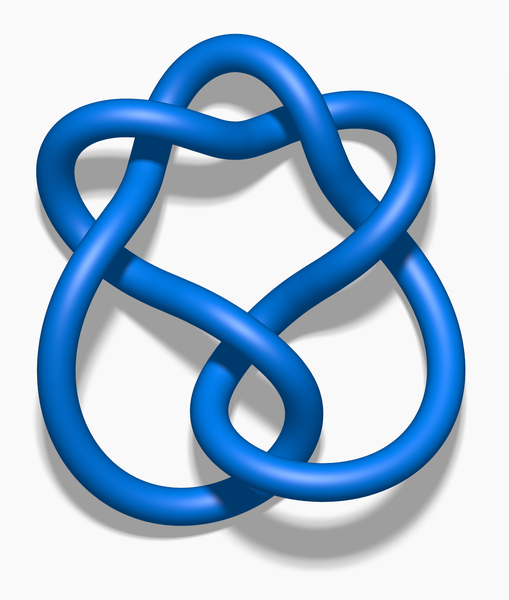
\includegraphics[width=0.7\textwidth]{./rozdzialy/6_1-3d.png}};

    \coordinate (a0) at (0,0);
    \coordinate (a1) at (90:5);
    \coordinate (a2) at (45:3);
    \coordinate (a3) at (-40:4.6);
    \coordinate (a4) at (-120:2.4);
    \coordinate (a5) at (10:0.7);
    \coordinate (a6) at (50:5);
    \coordinate (a7) at (90:3.5);
    \coordinate (a8) at (180-50:5);
    \coordinate (a9) at (170:0.7);
    \coordinate (a10) at (-70:2.4);
    \coordinate (a11) at (220:4.6);
    \coordinate (a12) at (180-45:3);

    %\foreach \i in {0,...,12} \fill (a\i) circle (2pt);

    \begin{knot}[
      clip width=20, 
      flip crossing=1,
      flip crossing=3,
      flip crossing=6
      ]
      \strand[thick, ->] (a1) to[out=0, in=90+45] (a2) to[out=-45, in=40] (a3);
      \strand[thick, ->] (a3) to[out=220, in=-90] (a4) to[out=90, in=200] (a5);
      \strand[thick, ->] (a5) to[out=20, in=-60] (a6);
      \strand[thick, ->] (a6) to[out=150, in=5] (a7);
      \strand[thick, ->] (a7) to[out=170, in=20] (a8);
      \strand[thick, ->] (a8) to[out=240, in=160] (a9);
      \strand[thick, ->] (a9) to[out=-20, in=90] (a10);
      \strand[thick, ->] (a10) to[out=-90, in=-40] (a11);
      \strand[thick, ->] (a11) to[out=140, in=180+45] (a12);
      \strand[thick, ->] (a12) to[out=45, in=180] (a1);
    \end{knot}

    %\node at (80: 5) {$A$};
    %\node at (-40:4) {$B$};
    %\node at (45:5.5) {$C$};
    %\node at (135:5.5) {$D$};
    %\node at (-1.5,0.1) {$E$};
    %\node at (220:4) {$F$};
    %
    %\node[bgnd] at (70:4.7) {$1$};
    %\node[bgnd] at (25:3.9) {$2$};
    %\node[bgnd] at (-90:3) {$3$};
    %\node[bgnd] at (90:0.5) {$4$};
    %\node[bgnd] at (110:4.7) {$5$};
    %\node[bgnd] at (180-25:3.9) {$6$};

    %\draw[dashed] (70: 4) circle (0.4);
    %\draw[dashed] (28: 3.1) circle (0.4);
    %\draw[dashed] (-90:3.5) circle (0.4);
    %\draw[dashed] (-90:0.15) circle (0.4);
    %\draw[dashed] (180-28:3.1) circle (0.4);
    %\draw[dashed] (110:4) circle (0.4);
  \end{tikzpicture}
  \caption{\label{fig:6_1:knot}Diagram of knot $6_1$.}
\end{figure}
$$A=\begin{pmatrix}
  -1 & 0 & 0 & 0 & 0 & 0 \\ 
  0 & -1 & 0 & 0 & 0 & 0 \\ 
  0 & 0 & t & 0 & 0 & 0 \\ 
  0 & 0 & 0 & t & 0 & 0 \\ 
  0 & 0 & 0 & 0 & -2t^{-2}+5t^{-1}-2 & 0 \\ 
  0 & 0 & 0 & 0 & 0 & 0 
\end{pmatrix}$$
which after reduction is
$$A'=
\begin{pmatrix}
  -2t^{-2}+5t^{-1}-2
\end{pmatrix}
$$
a $1\times 1$ matrix with the only term being the Alexander polynomial of $6_1$.

Using diagram in \cref{fig:9_46:knot} of $9_{46}$ it can be calculated that the Smith normal form of $D\phi$ is
\begin{figure}[h]\centering
  \begin{tikzpicture}[bgnd/.style={circle, fill=white, draw=white}]
    %\node[opacity=0.2] at (0,0) {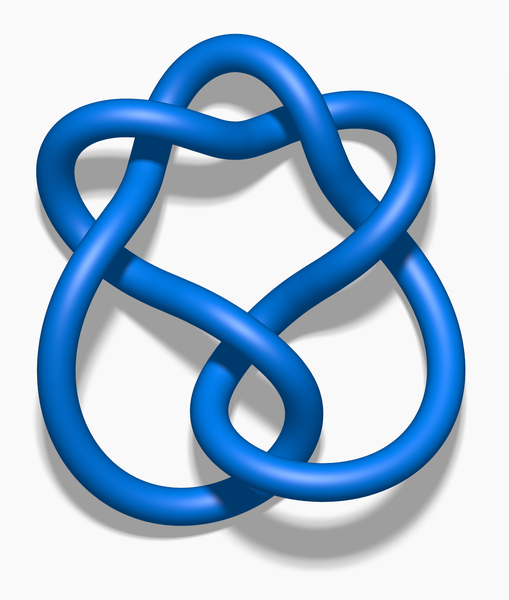
\includegraphics[width=0.7\textwidth]{./rozdzialy/6_1-3d.png}};

    \coordinate (a0) at (0,0);
    \coordinate (a1) at (60:5);
    \coordinate (a2) at (150:3);
    \coordinate (a3) at (-110:2.5);
    \coordinate (a4) at (-60:6);
    \coordinate (a5) at (30:1.5);
    \coordinate (a6) at (200:0.8);
    \coordinate (a7) at (170:5);
    \coordinate (a8) at (120:5);
    \coordinate (a9) at (30:3);
    \coordinate (a10) at (-70:2.5);
    \coordinate (a11) at (180+60:6);
    \coordinate (a12) at (150:1.5);
    \coordinate (a13) at (-20:0.8);
    \coordinate (a14) at (10:5);

    %\foreach \i in {0,...,14} \fill (a\i) circle (2pt);

    \begin{knot}[
      clip width=20, 
      consider self intersections,
      ignore endpoint intersections=false,
      %draft mode=crossings,
      flip crossing=1,
      flip crossing=4,
      flip crossing=7, 
      flip crossing=9
      ]
      \strand[thick, ->] 
        (a1) to [out=180, in=30]
        (a2) to [out=210, in=150]
        (a3);
      \strand[thick, ->]
        (a3) to [out=-30, in=180] 
        (a4) to [out=0, in=-15, looseness=1.5] 
        (a5);
      \strand[thick, ->]
        (a5) to [out=170, in=30] 
        (a6) to [out=220, in=-90] 
        (a7);
      \strand[thick, ->]
        (a7) to [out=90, in=180, looseness=1.3] 
        (a8) to [out=0, in=150] 
        (a9);
      \strand[thick, ->]
        (a9) to [out=-30, in=30]
        (a10) to [out=210, in=0] 
        (a11);
      \strand[thick, ->]
        (a11) to [out=180, in=180+15, looseness=1.5] 
        (a12) to [out=10, in=150]
        (a13);
      \strand[thick, ->]
        (a13) to [out=-40, in=-90]
        (a14) to [out=90, in=0, looseness=1.3]
        (a1);
      \fill[yellow] (-10:3.7) circle (6pt);
    \end{knot}
  \end{tikzpicture}
  \caption{\label{fig:9_46:knot}Diagram of knot $9_{46}$.}
\end{figure}
$$B=\begin{pmatrix}
  1 & 0 & 0 & 0 & 0 & 0 & 0 & 0 & 0 \\ 
  0 & t^{-1} & 0 & 0 & 0 & 0 & 0 & 0 & 0 \\ 
  0 & 0 & t^{-1} & 0 & 0 & 0 & 0 & 0 & 0\\ 
  0 & 0 & 0 & t  & 0 & 0 & 0 & 0 & 0 \\ 
  0 & 0 & 0 & 0 & t  & 0 & 0 & 0 & 0 \\ 
  0 & 0 & 0 & 0 & 0 & t  & 0 & 0 & 0\\ 
  0 & 0 & 0 & 0 & 0 & 0 & 2t-t^2 & 0 & 0 \\ 
  0 & 0 & 0 & 0 & 0 & 0 & 0 & t^{-2}-2t^{-1} & 0\\ 
  0 & 0 & 0 & 0 & 0 & 0 & 0 & 0 & 0
\end{pmatrix},$$
while reduced normal form of $D\phi$ is
$$B'=
\begin{pmatrix}
  2t-t^2 & 0 \\ 
  0      & t^{-2}-2t^{-1}
\end{pmatrix}
$$
which is significantly different than the one for $6_1$. Observe also that the determinant of both matrices is equal to the Alexander polynomial of corresponding knots 
$$\det(A')=-2+5t^{-1}-2t^{-2}$$
$$\det(B')=(2t-t^2)(t^{-2}-2t^{-1})=2t+2+2t^{-1}=-t(-2+5t^{-1}-2t^{-2}).$$
\marginnote{to wyliczenie wogóle jest na miejscu?} % TO DO
\end{example}

% {\large\color{red}TO DO: sprawdzić te węzły wyżej za pomocą pow. Seiferta, czy mają różne moduły Alexandera}

\begin{theorem}
  The reduced normal form of color checking matrix does not depend on the choice of diagram $D$. Thus, it is well defined for $K\phi$ and is a knot invariant.
\end{theorem}

\begin{proof}
  \marginnote{nie wiem, czy tutaj aż tak powinno się dokładnie mówić co i jak dodaję?} % TO DO
Take a knot $K$ and its diagram $D$ with $s$ segments and $x$ crossings. We will show that applying any Reidemeister move to this knot will not change the reduced normal form of its color checking matrix.

  \subsection*{\centering R1}

  The first Reidemeister move is split into \textbf{R1a} and \textbf{R1b}. Due to those two cases being analogous, we will focus on the move \textbf{R1a} (the proof of \textbf{R1b} is left as an exercise for the reader).

  Take $D'$ to be diagram $D$ with one arc twisted into a $+$ crossing. In opposition to the assumption in previous section, we will take the arcs and crossings that differ between those two diagrams to be on first positions. Now, the matrices $D\phi$ and $D'\phi$ are as follows
  $$
  D'\phi=
  \begin{bmatrix}
    b & a-1 & 0 & \hdots\\ 
    x_2 & y_2 & \hdots \\ 
    x_3 & y_3 \\ 
    \vdots 
  \end{bmatrix}
  $$
  $$
  D\phi=
  \begin{bmatrix}
    x_2 + y_2 & \hdots \\ 
    x_3 + y_3 \\ 
    \vdots
  \end{bmatrix}
  $$
  Adding the first column of $D'\phi$ to the second column will yield 
  $$
  D'\phi=
  \begin{bmatrix}
    b & 0 & 0 & \hdots\\ 
    x_2 & x_2+y_2 & \hdots \\ 
    x_3 & x_3+y_3 \\ 
    \vdots 
  \end{bmatrix}
  $$
  because $a+b=1$. Now we know that $b$ is a unit, thus we can easily remove the elements of the first column that are not $b$. This results in 
  $$
  D'\phi=
  \begin{bmatrix}
    b & 0 & 0 & \hdots\\ 
    0 & x_2+y_2 & \hdots \\ 
    0 & x_3+y_3 \\ 
    \vdots 
  \end{bmatrix}
  $$
  notice that the lower right portion of this matrix looks exactly like $D\phi$. The only difference is a column containing a singular unit element and thus it will be struck out when computing the reduced normal form. Thus, the reduced normal form of $D'\phi$ is the same as in $D\phi$.
  
  \subsection*{\centering R2}

  Now the diagram $D'$ is a diagram $D$ with one arc poked onto another. Once again we will put those changed arcs at the beggining of the color checking matrix to obtain following matrices:
  $$
  D'\phi=
  \begin{bmatrix}
    \alpha & \beta & -1 & 0 & \hdots \\ 
    a & 0 & b & -1  \\ 
    x_3 & u_3 & 0 & v_3 \\ 
    x_4 & u_4 & 0 & v_4 \\ 
    \vdots & & & & \ddots
  \end{bmatrix}
  $$
  $$
  D\phi= 
  \begin{bmatrix}
    x_3 & u_3 + v_3 & \hdots \\ 
    x_4 & u_4 + v_4 \\ 
    \vdots
  \end{bmatrix}
  $$
  Adding the third column of $D'\phi$ multiplied by $\alpha$ and $\beta$ to first and second column respectively we are able to reduce the first row to only zeros and $-1$. Now, adding this row to the second one creates a column with only $-1$ and zeros. We can put it as the first column:
  $$
  D'\phi=
  \begin{bmatrix}
    -1 & 0 & 0 & 0 & \hdots \\ 
    0 & a +b\alpha & 0 & -1  \\ 
    0 & x_3 & u_3 & v_3 \\ 
    0 & x_4 & u_4 & v_4 \\ 
    \vdots & & & & \ddots
  \end{bmatrix}
  $$
  Notice that $a+b\alpha=0$ and so we can transform this matrix into
  $$
  D'\phi=
  \begin{bmatrix}
    -1 & 0 & 0 & 0 & \hdots \\ 
    0 & -1 & -1 & 0  \\ 
    0 & v_3 +u_3 & v_3+u_3&  x_3 & \\ 
    0 & v_4 +u_4 & v_4+u_4 & x_4 \\ 
    \vdots & & & & \ddots
  \end{bmatrix}
  $$
  and then into 
  $$
  D'\phi=
  \begin{bmatrix}
    -1 & 0 & 0 & 0 & \hdots \\ 
    0 & -1 & 0 & 0  \\ 
    0 & 0 & v_3+u_3&  x_3 & \\ 
    0 & 0 & v_4+u_4 & x_4 \\ 
    \vdots & & & & \ddots
  \end{bmatrix}
  $$
  which obviously has the same reduced normal form as $D\phi$.

  \subsection*{\centering R3}

  $$D\phi=
  \begin{bmatrix}
    \alpha & -1 & \beta & 0 & 0 & 0 \\ 
    0 & 0 & -1 & b & 0 & a \\ 
    \beta & 0 & 0 & 0 & -1 & \alpha \\ 
    u_4 & 0 & v_4 & w_4 & x_4 & y_4
  \end{bmatrix}
  $$
  $$D'\phi=
  \begin{bmatrix}
    0 & 0 & -1 & \beta & \alpha & 0 \\ 
    \beta & 0 & 0 & 0 & -1 & \alpha \\ 
    0 & -1 & b & 0 & 0 & a\\ 
    u_4 & 0 & v_4 & w_4 & x_4 & y_4
  \end{bmatrix}
  $$

  Applying row and column operations on those matrices results in 
  $$
  D\phi=
  \begin{bmatrix}
    -1 & 0 & 0 & 0 & 0 & 0 \\
    0 & -1 & 0 & 0 & 0 & 0 \\ 
    0 & 0 & \beta & 0 & -1 & 0 \\ 
    0 & 0 & u_4+v_4 & w_4+v_4 & x_4-v_4 & y_4+u_4+x_4
  \end{bmatrix}
  $$
  $$
  D'\phi=
  \begin{bmatrix}
    b & 0 & 0 & 0 & 0 & 0 \\
    0 & -\beta & 0 & 0 & 0 & 0 \\ 
    0 & 0 & \beta & 0 & -1 & 0 \\ 
    0 & 0 & u_4+v_4 & w_4+v_4 & x_4-v_4 & y_4+u_4+x_4
  \end{bmatrix}
  $$
  which makes clear that those matrices have the same reduced normal form as $b$ and $\beta$ were taken to be units.

\end{proof}

